% äöüß
% by Torben Menke  http:/entorb.net
% date: 13.07.2019
% Copyright: Everyone using this template owes me a beer!

% PDF: 128 x 96 mm

% 1pt ~ 0.353mm !!!
% \paperwidth = 364.19536pt = 128.48003mm
% \textwidth = 307.28987pt = 108.40504mm
% \textheight = 219.85023pt = 77.558276 mm

% Done
% disable navigationsymbols on titlepage
% include Gnuplot -> MetaPost terminal plot example

\documentclass[
%   draft,          % placeholders instead of images, gray layout, FAST compiling!
  %handout,       % print-version without overlay-effects, problems when \only is used
  t,              % t / c all colums are aligned at top / center (default is c)
                  % can be set for each frame
  compress,       % make mini frames (navigations) as small as possible
  %11pt, % = default ?
  xcolor=dvipsnames,
  fragile, % for verbatim
  ]
  {beamer}

% Printversion
%\usepackage{pgfpages} \pgfpagesuselayout{4 on 1}[a4paper,border shrink=5mm,landscape]

\usepackage[ngerman]{babel} % ngerman
\usepackage[utf8]{inputenc}

\usepackage[T1]{fontenc}
%\usepackage{lmodern}

% TU Fonts, taken from tudmathposter_20110707

\pdfmapfile{=univers.map}
\pdfmapfile{=dinbold.map}

\usepackage[
,heavyfont % \seriesdefault = m instead of l
% ,serifmath % use serif font instead of CD font for math
]{beamerfontthemetud}

\usepackage{pgfpages} % for notes

% %Custom Footnotesymols
% \usepackage[perpage,symbol*]{footmisc} % perpage = reset counter on each page
% % Latex Default = \DefineFNsymbols*{lamport}{*\dagger\ddagger\S\P|{**}{\dagger\dagger}{\ddagger\ddagger}}
% \DefineFNsymbols*{TorbensFN}[math]{\ddagger\Sorg\P\dagger\ast{\dagger\dagger}{\ddagger\ddagger}{\ast\ast}{\Sorg\Sorg}{\P\P}}
% % \|
% % * wird nicht angezeigt und \S habe ich überschrieben, daher \Sorg
% \setfnsymbol{TorbensFN}
% % \setfnsymbol{wiley}
% 

% META DATA

%title[kurztitel]{titel}
% \title{Molecular Doping of Organic Semiconductors}
% \subtitle{A Conductivity and Seebeck Study}
\title[Molekulare Dotierung Organischer Halbleiter]{Molekulare Dotierung\\Organischer Halbleiter}
\subtitle{Eine Leitfähgkeits- und Seebeck-Studie}
\hypersetup{pdftitle={Molekulare Dotierung Organischer Halbleiter - Eine Leitfähgkeits- und Seebeck-Studie}}
\hypersetup{pdfsubject={Disputation, TU Dresden}}

\author[T. Menke]{Torben Menke}
\hypersetup{pdfauthor={Torben Menke}}
\date{19.07.2013}
\hypersetup{
pdfinfo={
CreationDate={D:20130719144500},
}
}

\newcommand*{\datecity}[1]{\renewcommand*{\insertdatecity}{#1}}
\providecommand*{\insertdatecity}{Dresden}

% \title[Title Kurzform]{Kompletter Titel}
% \subtitle[Untertitel Kurzform]{Untertitel}
% \author[T. Menke]{Torben Menke}
% \date[18.11.2010]{\insertdatecity{}, 18.11.2010}
% %\institute[IAPP - TU Dresden]{Institut für Angewandte Photophysik\\Technische Universität Dresden}
% %\titlegraphic{\includegraphics[width=3cm]{logo-iapp_white.pdf}}

% % PDF Stuff
%\subject{10$^\text{th}$ and last OSOL Work Presentation}
\keywords{Molecular Doping, Organic Semiconductors, Seebeck, Conductivity}
\hypersetup{pdfkeywords={Molecular Doping, Organic Semiconductors, Seebeck, Conductivity, Vacuum Deposition}}

\datecity{Disputation}

\usepackage{xspace}

\usepackage[
abbreviations = false
,noload={abbr} % \mm
,load={prefix,named,physical,accepted,addn} % no linebreaks or spacing here!
%prefix   \kilometer \milli
%named    \celsius \ohm \siemens
%physical \electronvolt
%accepted \degree \liter \percent
%addn     \BAR, \millibar, \angstrom
%,tabautofit
,tabnumalign=centredecimal % tabs: use S as collumn format -> center on '.'
,expproduct=tightcdot % cdot tightcdot times tighttimes
,per=frac,fraction=nice % \per now produces nice fractions
%,obeyfamily=true
%,obeyall=true
%,obeyitalic=false
%,obeybold=false
%,mode=text
,unitmode=text
%,mathsrm=mathsf
%,mathssf=mathsf
%,mathstt=mathsf
%,textrm=sffamily
%,textsf=sffamily
%,texttt=sffamily
%,inlinebold=text
]{siunitx} % Ubuntu 11.10 comes with version 1.3a (21.09.2009)

% \sisetup{obeyfamily=false,mathrm=mathsf,textrm=sffamily}

% \begin{textblock}{16}[0.0,0.0](10,78)
% \tiny Bild: Wikipedia
% \end{textblock}

% \begin{textblock}{20}[1,1](105,80)
% \includegraphics[page=3]{pics/Setup-ani-3D.pdf}%width=20mm
% \end{textblock}}

% \setlength{\TPHorizModule}{\paperwidth}\setlength{\TPVertModule}{\paperheight}
% After that, all the placing specifications can be referred to \TPHorizModule and TPVertModule. A typical use of textpos would be:
% 
% \begin{textblock}{width}[xt,yt](X,Y)  the-text-goes-here  \end{textblock}
% 
% where width is the desired width of the text box (the height will be enough to place all the text specified), X and Y are the (x,y) placement of the text box, and xt and yt are the point inside the text box which will be placed at (X,Y). All the units refer to \TPHorizModule and TPVertModule. For example:
% 
% \begin{textblock}{0.6}[0.5,0.5](0.3,0.4)  hello world\end{textblock}
% 
% will print the text “hello world” in a box of width 60% of \TPHorizModule (in my example, this is 60% of the total page width). The center (0.5,0.5) of that box will be placed at a point 30% to the right of the left margin, and 40% below the top margin (in TPxxxModule units).

\usepackage{ifthen}
%\ifthenelse{\equal{\tmDraft}{True}}%
%{}% True
%{}% False

%\usepackage[square,super,numbers,sort&compress]{natbib}     % needed by plainnat + dinat Bib Styls, square -> [] instead of () , numbers -> [1] etc

% THEME
% Source: http://www2.informatik.hu-berlin.de/~mischulz/beamer.html

\usetheme{Antibes}
% /usr/share/texmf/tex/latex/beamer/base/themes/theme/
% AnnArbor , Antibes , Bergen , Berkeley , Berlin , Boadilla , boxes , CambridgeUS , Copenhagen , Darmstadt , default , Dresden , Frankfurt , Goettingen ,Hannover , Ilmenau , JuanLesPins , Luebeck , Madrid , Malmoe , Marburg , Montpellier , PaloAlto , Pittsburgh , Rochester , Singapore , Szeged , Warsaw %\usetheme[height=13mm]{Rochester}

\useinnertheme{rounded}
% circles , default , inmargin , rectangles , rounded

% Transparent Overlays
%\setbeamercovered{transparent}

% Disable Navigationselements
\beamertemplatenavigationsymbolsempty

\setbeamertemplate{blocks}[rounded][shadow=false]

\newlength\Logoheight
\setlength\Logoheight{0.7cm}
% \pgfdeclareimage[height=\Logoheight,page=1]{logo-tu}{logo-tu_white.pdf}
% \pgfdeclareimage[height=\Logoheight,page=1]{logo-iapp}{logo-iapp_white.pdf}

% Faktor zur PPT-Vorlage: / 0,1984375      * 5,04

% Template infolines used: /usr/share/texmf/tex/latex/beamer/themes/outer
\defbeamertemplate{footline}{slides}%
{%
\usebeamercolor*{framefoot}%
\hbox{%
\hspace*{.02\paperwidth}%
\begin{beamercolorbox}[wd=.13\paperwidth,left ]{framefoot}\usebeamercolor*[fg]{framefoot}\insertshortdate\end{beamercolorbox}%
\begin{beamercolorbox}[wd=.70\paperwidth,center]{framefoot}\usebeamercolor*[fg]{framefoot}\insertshorttitle\end{beamercolorbox}%
\begin{beamercolorbox}[wd=.13\paperwidth,right]{framefoot}\usebeamercolor*[fg]{framefoot}\insertframenumber\end{beamercolorbox}%\insertpagenumber or \insertframenumber
}%
\vspace*{0.5ex}%
\hbox{%
\hspace*{.02\paperwidth}%
\begin{beamercolorbox}[wd=.13\paperwidth,left ]{framefoot}\usebeamercolor*[fg]{framefoot}\end{beamercolorbox}%
\begin{beamercolorbox}[wd=.70\paperwidth,center]{framefoot}\usebeamercolor*[fg]{framefoot}\insertauthor\end{beamercolorbox}%
\begin{beamercolorbox}[wd=.13\paperwidth,right]{framefoot}\usebeamercolor*[fg]{framefoot}\end{beamercolorbox}%
}%
\vspace{5pt}%
}

\defbeamertemplate{footline}{titlepage}{}

\setbeamertemplate{footline}[slides]%

\defbeamertemplate{headline}{titlepage}
{%
\vspace{2.3pt}%
\begin{beamercolorbox}[wd=1.0\paperwidth]{framehead}%,dp=0.1cm
\hspace*{.02\paperwidth}
\includegraphics[page=1,height=\Logoheight]{pics/logo-tu_white2.pdf}%
\hfill%
\includegraphics[page=1,height=\Logoheight]{pics/logo-iapp_white2.pdf}%
\hspace*{.02\paperwidth}
\end{beamercolorbox}%
\usebeamercolor*{framehead}%
\vspace*{2pt}%
\rule{\paperwidth}{0.5pt}\par
\hbox{%
\begin{beamercolorbox}[wd=.5\paperwidth,ht=2ex,dp=.5ex,center]{framehead}%
\usebeamerfont{section in head/foot}\bfseries%
\phant%
\end{beamercolorbox}%
\begin{beamercolorbox}[wd=.5\paperwidth,ht=2ex,dp=.5ex,left]{framehead}%
\usebeamerfont{subsection in head/foot}%
\phant%
\end{beamercolorbox}%
}\par%
\rule{\paperwidth}{0.5pt}\par%
% \vspace*{-2.70pt}% % weil warnung vbox too high
}%

\defbeamertemplate{headline}{intro}
{%
\vspace{2.3pt}%
\begin{beamercolorbox}[wd=1.0\paperwidth]{framehead}%,dp=0.1cm
\hspace*{.02\paperwidth}
\includegraphics[page=1,height=\Logoheight]{pics/logo-tu_white2.pdf}
\hfill%
\includegraphics[page=1,height=\Logoheight]{pics/logo-iapp_white2.pdf}
\hspace*{.02\paperwidth}
\end{beamercolorbox}%
\vspace*{2pt}%
\par
\usebeamercolor*[fg]{framehead}%
\rule{\paperwidth}{.5pt}\par%
\hbox{%
\begin{beamercolorbox}[wd=.5\paperwidth,ht=2ex,dp=.5ex,center]{framehead}%
\usebeamerfont{section in head/foot}\bfseries%
\phant%
\end{beamercolorbox}%
\begin{beamercolorbox}[wd=.5\paperwidth,ht=2ex,dp=.5ex,left]{framehead}%
\usebeamerfont{subsection in head/foot}%
\phant%
\end{beamercolorbox}%
}\par%
\usebeamercolor*[fg]{framehead}%
\rule{\paperwidth}{0.5pt}\par%
% \vspace*{-1.89pt}% % weil warnung vbox too high
}%

\defbeamertemplate{headline}{slides}
{%
\vspace{2.3pt}%
\begin{beamercolorbox}[wd=1.0\paperwidth]{framehead}%,dp=0.1cm
\hspace*{.02\paperwidth}
\includegraphics[page=1,height=\Logoheight]{pics/logo-tu_white2.pdf}
\hfill%
\includegraphics[page=1,height=\Logoheight]{pics/logo-iapp_white2.pdf}
\hspace*{.02\paperwidth}
\end{beamercolorbox}%
\vspace*{2pt}%
\par
\usebeamercolor*[fg]{framehead}%
\rule{\paperwidth}{.5pt}\par%
\hbox{%
\begin{beamercolorbox}[wd=.5\paperwidth,ht=2ex,dp=.5ex,center]{framehead}%
\usebeamerfont{section in head/foot}\bfseries%
\insertsectionnavigationhorizontal{0.5\paperwidth}{\hskip0pt plus1filll}{}%
\end{beamercolorbox}%
\begin{beamercolorbox}[wd=.5\paperwidth,ht=2ex,dp=.5ex,left]{framehead}%
\usebeamerfont{subsection in head/foot}%
\insertsubsectionnavigationhorizontal{0.5\paperwidth}{}{\hskip0pt plus1filll}%
\end{beamercolorbox}%
}\par%
\usebeamercolor*[fg]{framehead}%
\rule{\paperwidth}{0.5pt}\par%
% \vspace*{-1.89pt}% % weil warnung vbox too high
}%

\defbeamertemplate{frametitle}{slides}
{%
\begin{textblock}{87}[0.5,0.0](71,3)% {3} (0,0) % 87mm wide, (pagewidth=128mm), 3mm border to page top, [0.5,0.0] = center in x, top in y
\centering%
\insertframetitle\phant% Phant = Zeichen"fp" damit alle Boxen gleich hoch sind
\end{textblock}%
\vspace*{-2.6pt}% bei diesem wert ist die erste Zeile einer Folie mit titel an der selben stelle wie die einer Folie ohne titel, warum auch immer
}

\defbeamertemplate*{title page}{titlepage}{
\vfill\vfill%
{
\usebeamerfont*{title}%
\inserttitle%
\par%
}%
\vfill%
{%
\ifx\insertsubtitle\empty
\else
\usebeamerfont*{subtitle}\insertsubtitle
\vfill
\vfill
\scriptsize \insertauthor % by 
\fi%
\vfill\scriptsize\insertdatecity, \insertdate
}%
\vfill%
\begin{textblock*}{2cm}[0,0](90mm,28mm) % Seite: 128mm x 96mm
\includegraphics{pics/titel-spritze.pdf} % width=2cm
\end{textblock*}
}

\renewcommand\maketitle{%
\setbeamertemplate{headline}[titlepage]%
\setbeamertemplate{footline}[titlepage]%
\frame{\titlepage}
\setbeamertemplate{headline}[intro]%
% \setbeamertemplate{headline}[slides]% Later, manually after Intro
\setbeamertemplate{footline}[slides] % does not work here, so later...
\setbeamertemplate{frametitle}[slides]
\setbeamertemplate{note page}[TorbensNotizen]
}%

\renewcommand{\footnoterule}{} % remove ruler above footnotes


% % Farbdefinitionen aus tudbeamer vorlage
% %\definecolor{tublau}{RGB}{0,29,75} % aus OpenOffice Vorlage -> sieht falsch aus, daher cmyk
% \definecolor{tublau}{cmyk}{0.86,0.48,0,0.68} % aus OpenOffice Vorlage

% aus TUD Farbregister
\definecolor{tublau100}{HTML}{0B2A51}
\definecolor{tublau90}{HTML}{1D355B}
\definecolor{tublau80}{HTML}{2F4067}
\definecolor{tublau70}{HTML}{4C7AB9}
\definecolor{tublau60}{HTML}{6185C0}
\definecolor{tublau50}{HTML}{7392C9}
\definecolor{tublau40}{HTML}{87A1D2}
\definecolor{tublau30}{HTML}{9CB1DB}
\definecolor{tublau20}{HTML}{B8C6E6}
\definecolor{tublau10}{HTML}{D8E0F2}
\definecolor{tuauszeich1}{HTML}{0059A3}%blau
\definecolor{tuauszeich180}{HTML}{346FB2}%blau 80%
\definecolor{tuauszeich140}{HTML}{87A1D2}%blau 80%
\definecolor{tuauszeich2}{HTML}{51297F}%dk lila
\definecolor{tuauszeich250}{HTML}{B07CAE}%dk lila
\definecolor{tuauszeich3}{HTML}{811A78}%magenta
\definecolor{tuauszeich4}{HTML}{007A47}%grün

\definecolor{tublau}{HTML}{0B2A51} % tublau100

% Eigene Latex Farben für Mat Namen
\definecolor{CrPd}{HTML}{FF98FF}
\definecolor{WPd}{HTML}{00FF00}
\definecolor{DMBI}{HTML}{FF9D00}
\definecolor{AOB}{HTML}{00FFFF}
% {0,1,0}

% 
% % Farbdefinitionen aus TUBeamervorlage
% \definecolor{tuwhite}{gray}{1.00}
% \definecolor{tublack}{gray}{0.00}
% \definecolor{tuskyblue}{rgb}{0.80, 0.80, 1.00}
% \definecolor{tublue}{rgb}{0.20, 0.20, 0.80}
% \definecolor{tudarkblue}{rgb}{0.04, 0.16, 0.32}
% % \definecolor{extradarkblue}{rgb}{0.00, 0.15, 0.36}
% \definecolor{tuextradarkblue}{cmyk}{1.00, 0.70, 0.10, 0.50}
% \definecolor{tuturquoise}{rgb}{0.00, 0.80, 0.60}
% \definecolor{tugray}{gray}{0.59}
% \definecolor{tudarkgray}{gray}{0.50}
% 

%
% \definecolor{HKS92K100}{cmyk}{0.1,0.00,0.05,0.65}
%
% \definecolor{HKS44K100}{cmyk/rgb}{1.00,0.50,0.0,0.0/0,0.34902,0.639216}
% \colorlet{alert}{HKS44K100}
%

\setbeamercolor{normal text}{fg=white,bg=tublau}

\setbeamercolor{note text}{fg=black,bg=white}

%
%
\setbeamercolor{structure}{fg=tublau50,bg=tublau}
%
\setbeamercolor{framefoot}{fg=gray,bg=tublau}
\setbeamercolor{framehead}{fg=white,bg=tublau}
% %
% %
% %
% % % meine Grafiken kommen in solch eine Box
\setbeamercolor{colorfigurebox}{fg=tublau,bg=white}

% \setbeamercolor*{block body title}{bg=red,fg=white}

\setbeamercolor{block title}{bg=tuauszeich1,fg=white}
\setbeamercolor{block body}{bg=tublau80,fg=white}

% \setbeamercolor{item projected}{bg=tuauszeich2,fg=white}

%  \setbeamercolor{section number projected}{bg=tuauszeich2,fg=white}
\setbeamerfont  {section number projected}{family=\sffamily,series=\mdseries,size=\normalsize}

% Analog block body, title, example etc.

% \setbeamercolor*{separation line}{fg=white}
% \setbeamercolor{section in head/foot}{fg=white,bg=tublau}
% \setbeamercolor{subsection in head/foot}{fg=white,bg=tublau}
% \setbeamercolor*{author in head/foot}{fg=white,bg=tublau}
% \setbeamercolor*{title in head/foot}{fg=white,bg=tublau}
% \setbeamercolor*{date in head/foot}{fg=white,bg=tublau}
% \setbeamercolor*{titlelike}{fg=white,bg=tublau}

% \setbeamercolor*{palette primary}{fg=white,bg=tublau}
% \setbeamercolor*{palette secondary}{fg=white,bg=tublau}
% \setbeamercolor*{palette tertiary}{fg=white,bg=tublau}
% \setbeamercolor*{palette quaternary}{fg=white,bg=tublau}

% notes
%\setbeameroption{show notes}
%\setbeameroption{show notes on second screen=right}
% notes:
%/usr/share/texmf/tex/latex/beamer/base/beamerbasenotes.sty

% % custom note page
% % http://blog.hartwork.org/?p=1466
% \setbeamertemplate{note page}{%
% \insertnote%
% }
% \newlength{\parskipbackup}
% \setlength{\parskipbackup}{\parskip}
% \newlength{\parindentbackup}
% \setlength{\parindentbackup}{\parindent}
% \let\notebackup\note
% \renewcommand{\note}[1]{\notebackup{%
% \mode<handout>{\addtocounter{page}{-1}}%
% \setlength{\parindent}{0ex}%
% \setlength{\parskip}{10pt}%
% \noindent%
% {\normalsize{}#1}%
% \setlength{\parskip}{\parskipbackup}%
% \setlength{\parindent}{\parindentbackup}%
% }%

\hypersetup{
pdfstartview={Fit}
,pdfpagemode={UseNone} % UseOutlines, UseThumbs, UseNone, FullScreen
,pdfpagelayout={SinglePage} % SinglePage, OneColumn, TwoPageLeft, TwoPageRight}
}

\usepackage[
absolute
,overlay
% ,showboxes
]{textpos}
% set unit of mea
\setlength{\TPHorizModule}{1mm} \setlength{\TPVertModule}{\TPHorizModule}

\begin{document}
% geo: 128mm x 96mm

\newcommand{\grad}[1] {\SI{#1}{\celsius}}
\newcommand{\K}[1] {\SI{#1}{\kelvin}}
\newcommand{\Scm} [1] {\SI[per=frac,fraction=nice,valuesep=thick]{#1}{\siemens\per\centi\meter}}
\newcommand{\mV}  [1] {\SI{#1}{\milli\volt}}
\newcommand{\V}  [1] {\SI{#1}{\volt}}
\newcommand{\meV} [1] {\SI{#1}{\milli\electronvolt}}
\newcommand{\nm} [1] {\SI{#1}{\nano\meter}}
\newcommand{\mm} [1] {\SI{#1}{\milli\meter}}
\newcommand{\uVK} [1] {\SI{#1}{\mu\volt\per\kelvin}} % \micro -> Font eurm10 at 10pt not found
\newcommand{\cmVs}  [1] {\SI{#1}{\centi\meter\squared\per\volt\per\second}}
\newcommand{\mr}[1] {\SI{#1}{MR}}

\newcommand{\vs}[0] {vs.\ }
\newcommand{\etal}[0] { \mbox{et al.}\xspace}
\newcommand{\insitu}[0] {in~situ\xspace}

\newcommand{\phant}[0]{\hspace*{-2ex}\phantom{fg}} % invisible box for fixing jumping text

\newcommand{\pfeil} [0] {\ensuremath{\rightarrow}\xspace}
\newcommand{\Pfeil} [0] {\ensuremath{\Rightarrow}\xspace}

% \renewcommand{\thefootnote}{\fnsymbol{footnote}}

% \newcommand{\zitat} [1] {\footnote{\tiny{#1}}}
\newcommand{\zitat} [1] {\fnSym\fn{#1}}
\newcommand{\fnSym}[0]{\ensuremath{^\ast}} % \ast is schlecht weil in Gleichung verwendet
\newcommand{\fn} [1] {%
\begin{textblock}{108}[0.0,0.0](10,85)
\tiny{\fnSym#1}%
\end{textblock}%
}

% \newcommand{\cond} [0] {\ensuremath{\sigma}\xspace}
\let\corg\c
\renewcommand{\c} [1][\empty]%
{%
\ifthenelse{\equal{#1}{\empty}}%
{\ensuremath{\sigma}\xspace}%
{\mbox{\ensuremath{\sigma=\Scm{#1}}}}%
}
\newcommand{\C} [1][\empty]%
{%
\ifthenelse{\equal{#1}{\empty}}%
{\ensuremath{C}\xspace}%
{\mbox{\ensuremath{C=#1}}}%
}

\newcommand{\Eact} [1][\empty]{\ifthenelse{\equal{#1}{\empty}}%
 {\texorpdfstring{\ensuremath{E_\text{act,\c}}}{Eact}\xspace}%
 {\mbox{\ensuremath{E_\text{act,\c}=\meV{#1}}}}%
}
% \newcommand{\Eact} [0] {\texorpdfstring{\ensuremath{E_\text{act,\c}}}{Eact}\xspace}
\newcommand{\Es} [1][\empty]{\ifthenelse{\equal{#1}{\empty}}%
 {\ensuremath{E_\text{S}}\xspace}%
 {\mbox{\ensuremath{E_\text{S}=\meV{#1}}}}%
}
\newcommand{\Et} [1][\empty]{\ifthenelse{\equal{#1}{\empty}}%
 {\ensuremath{E_\text{Tr}}\xspace}%
 {\mbox{\ensuremath{E_\text{Tr}=\meV{#1}}}}%
}
\newcommand{\Ef} [0] {\ensuremath{E_\text{F}}\xspace}
\newcommand{\Ec} [0] {\ensuremath{E_\text{C}}\xspace}
\newcommand{\Ev} [0] {\ensuremath{E_\text{V}}\xspace}
\newcommand{\Egap} [0] {\ensuremath{E_\text{gap}}\xspace}
\newcommand{\kB} [0] {\ensuremath{k_\text{B}}\xspace}
\newcommand{\kT} [0] {\ensuremath{\kB T}\xspace}
\newcommand{\Tm} [0] {\ensuremath{T_\text{m}}\xspace}
\newcommand{\Tmess} [1][\empty]{\ifthenelse{\equal{#1}{\empty}}%
 {\ensuremath{T_\text{Mess}}\xspace}%
 {\mbox{\ensuremath{T_\text{Mess}=\grad{#1}}}}%
}
\newcommand{\T} [1][\empty]{\ifthenelse{\equal{#1}{\empty}}%
 {\ensuremath{T}\xspace}%
 {\mbox{\ensuremath{T=\grad{#1}}}}%
}
\let\Sorg\S
\renewcommand{\S} [0] {\ensuremath{S}\xspace}

\newcommand{\dos}     [0] {\ensuremath{D}\xspace}

\newcommand{\DopEff} [1][\empty]{\ifthenelse{\equal{#1}{\empty}}%
 {\ensuremath{\eta_\text{dot}}\xspace}%
 {\mbox{\ensuremath{\eta_\text{dot}=\SI{#1}{\percent}}}}%
}
\newcommand{\DopEffLL} [1][\empty]{\ifthenelse{\equal{#1}{\empty}}%
 {\ensuremath{\eta_\text{dot,min}}\xspace}%
 {\mbox{\ensuremath{\eta_\text{dot,min}=\SI{#1}{\percent}}}}%
}
\newcommand{\mob}  [1][\empty]{\ifthenelse{\equal{#1}{\empty}}%
 {\ensuremath{\mu}\xspace}%
 {\mbox{\ensuremath{\mu=\cmVs{#1}}}}%
}
\newcommand{\mobLL}  [1][\empty]{\ifthenelse{\equal{#1}{\empty}}%
 {\ensuremath{\mu_\text{min}}\xspace}%
 {\mbox{\ensuremath{\mu_\text{min}=\cmVs{#1}}}}%
}
\newcommand{\mobUL}  [1][\empty]{\ifthenelse{\equal{#1}{\empty}}%
 {\ensuremath{\mu_\text{max}}\xspace}%
 {\mbox{\ensuremath{\mu_\text{max}=\cmVs{#1}}}}%
}
\newcommand{\n} [0] {\ensuremath{n_\text{e}}\xspace}
\newcommand{\nLL} [0] {\ensuremath{n_\text{min}}\xspace}

\newcommand{\nM} [0] {\ensuremath{n_\text{Mol}}\xspace}
\newcommand{\nH} [0] {\ensuremath{n_\text{W}}\xspace}
\newcommand{\nD} [0] {\ensuremath{n_\text{D}}\xspace}

\newcommand{\fFD}     [0] {\ensuremath{f_\text{FD}}\xspace}
\newcommand{\gausswidth} [1][\empty]{\ifthenelse{\equal{#1}{\empty}}%
 {\ensuremath{\sigma_\text{G}}\xspace}%
 {\mbox{\ensuremath{\sigma_\text{G}=\meV{#1}}}}%
}

\newcommand{\gausscenter} [0] {\ensuremath{E_\text{G}}\xspace}

\newcommand{\meo} [0] {MeO-TPD\xspace}
\newcommand{\lili} [0] {BF-DPB\xspace}
\newcommand{\CSF} [0] {\texorpdfstring{C$_{60}$F$_{36}$}{C60F36}\xspace}
\newcommand{\FS} [0] {\texorpdfstring{F$_{6}$-TCNNQ}{F6TCNNQ}\xspace}

\newcommand{\AS} [0] {\textcolor{AOB}{luft}\textcolor{DMBI}{stabile}\xspace}
\newcommand{\Pd} [0] {\textcolor{CrPd}{luft}\textcolor{WPd}{reaktive}\xspace}
\newcommand{\CS} [0] {\texorpdfstring{C$_{60}$}{C60}\xspace}
\newcommand{\aob} [0] {\textcolor{AOB}{AOB}\xspace}
\newcommand{\CrPd}[0] {\textcolor{CrPd}{Cr$_2$(hpp)$_4$}\xspace} %Magenta
\newcommand{\WPd} [0] {\textcolor{WPd}{W$_2$(hpp)$_4$}\xspace}
\newcommand{\aobLong} [0] {3,6-bis(dimethylamino)acridine\xspace}
\newcommand{\dmbiPOHLong}[0] {2-(1,3-dimethyl-1\textsl{H}-benzoimidazol-3-ium-2-yl)phenolatehydrate\xspace}
\newcommand{\CrPdLong}[0] {tetrakis(1,3,4,6,7,8-hexahydro-2H-pyrimido[1,2-a]pyrimidinato)dichromium (II)\xspace}
\newcommand{\WPdLong}[0]  {tetrakis(1,3,4,6,7,8-hexahydro-2H-pyrimido[1,2-a]pyrimidinato)ditungsten (II)\xspace}
\newcommand{\dmbiPOH}[0] {\textcolor{DMBI}{DMBI-POH}\xspace}
\newcommand{\dmbi}[0] {\dmbiPOH}

% redefine the section
% \let\sectionorg\section % damit keine endlosschleife erzeugt wird
% \renewcommand{\section}[1]{\sectionorg{#1}\einzeiler{\huge\bfseries\thesection. #1}}
% \let\subsectionorg\subsection % damit keine endlosschleife erzeugt wird
% \renewcommand{\subsection}[1]{\subsectionorg{#1}\einzeiler{\large\bfseries\thesection.\thesubsection{} #1}}

% [1]=width colum1
% {2}=column1, {3}=column2
\newdimen\SpalteL%
\newdimen\SpalteR%

\newcommand{\spalten}[3][0.5\textwidth]{%
\SpalteL=0mm%
\SpalteR=0mm%
\advance\SpalteL by #1 %
\advance\SpalteR by \textwidth %
\advance\SpalteR by -\SpalteL %
\begin{columns}[T]%t/c/T alignment
\begin{column}{\SpalteL}%
#2%
\end{column}%
\begin{column}{\SpalteR}%
#3%
\end{column}%
\end{columns}%
}

\newcommand{\spaltenC}[3][\empty]{% Zentriert
\SpalteL=0mm%
\SpalteR=0mm%
\ifthenelse{\equal{#1}{\empty}}%
{\advance\SpalteL by 0.5\textwidth}
{\advance\SpalteL by #1}%
\advance\SpalteR by \textwidth%
\advance\SpalteR by -\SpalteL%
\begin{columns}[T]%t/c/T alignment
\begin{column}{\SpalteL}%
\centering%
#2%
\end{column}%
\begin{column}{\SpalteR}%
\centering%
#3%
\end{column}%
\end{columns}%
}

% \einzeiler[title]{text}
\newcommand{\einzeiler}[2][\empty]{%
\begin{frame}[c]
\begin{center}
\frametitle{#1\phant} \phant#2\phant
\end{center}
\end{frame}
}

%\todoframe[title]{Slope of Cond}
\newcommand{\todoframe}[1]{% [2][TODO]
\einzeiler{\textcolor{red}{\bfseries \Large TODO: #1}}
}

\newcommand{\todo}[1]{%
\begin{textblock}{128}[1.0,0.0](128,0)%
\tiny{\phant\textcolor{yellow}{\hfill TODO: #1}}%
\end{textblock}
}

\newcommand{\ton}[1]{%
\begin{textblock}{128}[0.0,1.0](0,95.5)%
\tiny{\phant\textcolor{yellow}{Ton: #1}}%
\end{textblock}
}

\newcommand{\bildbox}[3][scaled]{% [1]=unscaled  2=file; 3=width
% Achtung: rounded=true -> box + 4pt in jeder Richtung
\begin{beamercolorbox}[center,rounded=true,shadow=false,wd=#3]{colorfigurebox}%
\centering%
\ifthenelse{\equal{#1}{unscaled}}%
{\includegraphics[page=1]{#2}}%
{\includegraphics[page=1,width=#3]{#2}}%
\end{beamercolorbox}%
}

\newcommand{\bildframe}[4][scaled]{% [1]=unscaled  2=title 2=file; 3=width
\begin{frame}{#2}%
\bildbox[#1]{#3}{#4}%
\end{frame}%
}

\newdimen \boxbreite %wird dann gesetzt
\newcommand{\calcBoxBreite}[1]{% 1=wunschbreite
\boxbreite=#1%
\advance\boxbreite by -8pt % leer hier wichtig! rahmen bei rounded=true= 2x 4pt
%\the \boxbreite%
}

%calculate box width from given imagewidth
%\newdimen\boxbreite%
%\boxbreite=#1
%\advance\boxbreite by \boxrahmen % leer hier wichtig!
%\advance\boxbreite by \boxrahmen % leer hier wichtig!
%Ergebnis: \the\boxbreite

% tableofcontents-Options
% currentsection
% currentsubsection
% firstsection=⟨section number⟩ specifies which section should be numbered as section "1"
% hideallsubsections
% hideothersubsections
% part=⟨part number⟩ causes the table of contents of (part number) to be shown, instead of the
% table of contents of the current part
% pausesections pause before each secton
% pausesubsections pause before each subsecton
% sectionstyle=show/shaded  -> specifies how sections should be displayed. show,shaded,hide
% subsectionstyle=show/shaded/hide
% subsubsectionstyle

% DIES IST DIE URSACHE FÜR Acrobat Absturz!!!
% \AtBeginSection[] % Do nothing for \section*
% {%
% \einzeiler{\textcolor{white}{\bfseries \Large \thesection{}. \secname}}%kein plan warum textcolor entscheident ist...
% %\thesection{}.
% }
% \AtBeginSubsection[] % Do nothing for \subsection*
% {%
% \einzeiler{\textcolor{white}{\bfseries \large \thesection{}.\thesubsection{} \subsecname}}%kein plan warum textcolor entscheident ist...
% %\thesection{}.\thesubsection{}
% }

% Show the Outline at the beginning of every section
% \AtBeginSection[] % Do nothing for \section*
% {
% \begin{frame}[c]%
% \bfseries\Large%
% \begin{beamercolorbox}[wd=1.0\textwidth,ht=2.25ex,dp=1.0ex,center]{framehead}% ht=2.25ex,dp=1.0ex -> always same size
% %\thesection{}.
% \secname\phant
% \end{beamercolorbox}\par
% % \frametitle{Outline}
% %\tableofcontents[currentsection] %,hideallsubsections
% \end{frame}
% }

% \AtBeginSubsection[] % Do nothing for \subsection*
% {
% \begin{frame}[c]%
% \bfseries\large%
% \begin{beamercolorbox}[wd=1.0\textwidth,ht=2.25ex,dp=1.0ex,center]{framehead}%
% %\thesection{}.\thesubsection{}
% \subsecname\phant
% \end{beamercolorbox}\par
% \end{frame}
% }

% \einzeiler{\textcolor{red}{\bfseries \Large TODO: #1}}
\maketitle

%\renewcommand{\todoframe}[1]{}
%\renewcommand{\todo}[1]{}
%\renewcommand{\ton}[1]{}


\newcommand{\secbild}[0]{}
\renewcommand{\todo}[1]{}
\renewcommand{\ton}[1]{}

% % äöüß
\chapter{Introduction}
\addcontentsline{lof}{chapter}{\thechapter\hspace*{1ex} Introduction}
%
The second half of the 20$^\text{th}$ century was characterized by the advance of semiconductor electronics that led to the invention of computers, affecting most parts of today's daily life.
Most commonly the semiconductor material silicon is used, being the second most abundant element in the Earth's crust and having already been used for fabrication of ordinary glass for centuries.
One of the key elements that enabled the breakthrough of semiconductor technology is doping, \ie the introduction of electron donating or accepting impurities that allow for controlling of the majority charge carriers. Doping enables the design of p-n-junctions, being the building block for most electronic devices, from transistors to light-emitting diodes and photovoltaic cells. Furthermore, it allows for adjusting the conductivity over orders of magnitude by increasing the charge carrier density and therefore tuning charge injection, extraction and transport properties.

Recently, semiconductors composed of chemically synthesized organic (\ie hydrocarbon-based) molecules increasingly gained attention, since organic dyes with delocalized $\pi$-systems have promising properties for optoelectronic devices.
The major drawback of organic semiconductors is their rather low charge carrier mobility, being several orders of magnitude below the values of typical conventional semiconductors. This is due to the weak interaction between adjacent organic molecules in a layer that leads to a slower charge-transfer between the molecules, compared to the almost unhindered band transport in a crystalline inorganic semiconductor formed by covalently bound atoms.
%
But, whereas a limited variety of conventional (inorganic) semiconductor materials is available, the toolbox of organic chemistry allows to design and synthesize molecules with desired properties.

The optoelectronic properties of organic semiconductors led to the development of organic light-emitting diodes (OLED) and organic photovoltaic cells (OPV), converting electricity to light and vice versa. The lower refractive index of organic semiconductors compared to conventional semiconductors allows for good light in- and outcoupling. In the last 15\,years, the development of both technologies was accompanied by an exponentially increasing number of publications over time that drove exponentially increasing record efficiencies, as shown in \figref{oled+opv-pub+eff}.
In contrast to conventional electronics, both types of devices, OLEDs and OPV, can in principle be fabricated on foils allowing for flexible lightweight devices and large device areas, which opens new areas of applications.
The main drawback is that device lifetime is limited by reactions with water and oxygen, requiring exceptionally good encapsulation.
Device thicknesses in the range of just hundred nanometers and low fabrication temperatures with typical substrate temperatures below \grad{100} lead to very low material and energy consumption and hence promise low production costs.

\begin{wrapfigure}[32]{r}[5mm]{62.8mm}% width aus grafic auslesen
\vspace*{-0.5cm}
% #1=lines #2=placement #3=overhang into margin # 4=width
{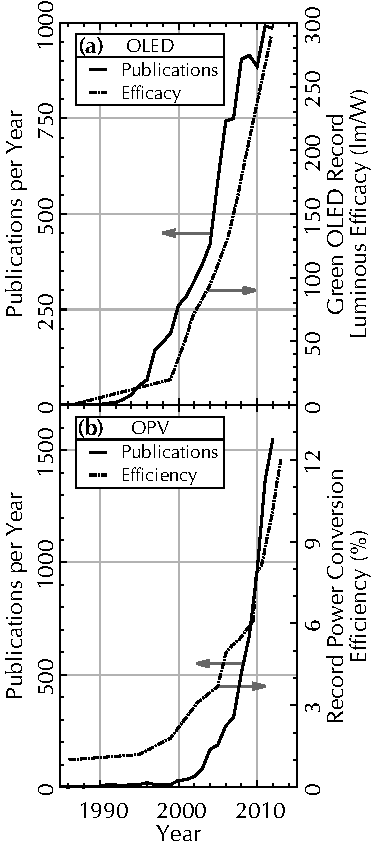
\includegraphics{plot/oled+opv-pub+eff}}
\caption
[OLED and OPV publications per year and laboratory ``hero'' performance]
{(a) OLED and (b) OPV publications per year and laboratory ``hero'' performance.\cite{OW,ISI}
}
\label{fig:oled+opv-pub+eff}
\end{wrapfigure}%
%
%
OLEDs are developed for lighting as well as for display applications.
OLED lighting competes with fluorescent lighting as well as inorganic light-emitting diode (LED) technology.
%
While LEDs are usually point light sources, OLEDs are natural area emitters of diffuse light and allow for new design options like transparent lighting panels. At the time of writing, first products are commercially available.
%
OLEDs for display applications have already proven their potential and successfully emerged into markets where they are competing with conventional liquid crystal display (LCD) technology. Key advantages of OLED displays are higher contrast, potentially low power consumption, smaller thickness and larger viewing angle, mostly enabled by the direct emission of light with the desired color instead of a combination of white backlight and color filters like in LCDs.

Organic semiconductor-based photovoltaics is a promising candidate for providing future electricity supply. Besides silicon-based photovoltaics, it seems to be the only non-concentrated technology with sufficient raw material available for a TW-scale production\cite{Feltrin2008}, required for a significant share of worldwide supply of sustainable electricity.
While for silicon-based photovoltaics the record efficiencies stagnated in recent years and only the production costs could be dramatically reduced, in the last 15 years exponentially increasing OPV record efficiencies have been reported, as shown in \figref{oled+opv-pub+eff}\,(b).
%
At the time of writing, a record power conversion efficiency of 12\,\%\cite{Heliatek12.0} 
is published which is below the record for polycrystalline silicon cells (20.4\,\%)\cite{SolarCellEff41} but already above the value for amorphous silicon (10.1\,\%)\cite{SolarCellEff41}.
In contrast to inorganic cells, the efficiency is stable between room temperature and elevated operating temperature and a better low-light performance is reported \cite{Riede2011,Heliatek12.0}.
%
The major drawback for polycrystalline silicon-based photovoltaic modules is the rather long energy payback time (\eg $\approx 2$ years when installed in Germany\cite{PV-Fakten201303}). Roll-to-roll processing of OPV modules on flexible substrates might allow for a high production throughput and hence, together with low material consumption and low fabrication temperatures, enable short energy payback time and low cost\cite{Anctil2012}.
Furthermore, the narrow absorption bands of organic semiconductors allow for fabrication of color-tunable semi-transparent cells as well as for efficiency-optimized tandem or triple cells\cite{Riede2011,Heliatek12.0}.

Two classes of organic semiconductors are typically distinguished: polymers and small molecules.
Polymers are large molecules consisting of repeating structural units and are typically deposited by wet chemical methods like coating or printing from solution. They show higher charge carrier mobilities than small molecules due to their intra-molecular transport, but chain length dispersity and solvent contamination hamper reproducibility.
Small molecules are compounds of rather low molar mass, often allowing for purification and deposition by thermal evaporation, typically in vacuum. Charge carrier mobilities are usually lower than in polymers and the initial cost for large scale production by vacuum deposition tends to be larger compared to solution processing of polymers. However, the thermal evaporation process allows for freely designable multilayer devices, which is hardly possible for polymers, due to the interaction of solvents with layers already deposited and the lack of orthogonal solvents.

Organic semiconductors can be doped by co-depositing electron donating or accepting atoms or molecules along with the host material. Doping of organic semiconductors has been shown to improve device performance significantly\cite{Walzer2007,LuessemRiedeLeo2013-PSS}, but contrary to conventional semiconductors, the underlying physics is far from being completely understood.
It is the aim of this thesis to contribute to the understanding of the fundamental physics of doping of organic semiconductors by studying the molecular doping in vacuum deposited layers of organic small molecules.

This thesis is structured into nine chapters. Following this introduction, chapter~\ref{chap:Theo} provides the theoretical background and reviews relevant literature for the studies presented in the subsequent chapters. In chapter~\ref{chap:Exp},
the experimental techniques as well as the developed setup are explained in detail. Furthermore, the investigated organic compounds are introduced and their key properties along a draft historical background are summarized.
The presentation of the results starts in chapter~\ref{chap:PaddleWheels} with investigations of the fullerene \CS n-doped by the two novel dopants \CrPd and \WPd of extremely low \IEs and which hence are reactive to air. The degradation induced by air-exposure of doped layers is studied and a regeneration treatment is presented.
In chapter~\ref{chap:AirStables}, \CS is n-doped by air-stable precursor compounds (\aob, \dmbi and \meodmbiI) that form the active dopant compound during deposition. This transformation is investigated more closely for the two novel DMBI derivatives.
Following the studies of n-doping, in chapter~\ref{chap:P-Doping} two amorphous hosts (\meo and \lili) are p-doped by two different dopants (\FS and \CSF) and the influence of the molecular energy levels on the doping is analyzed.
Afterwards, in chapter~\ref{chap:P5} the model system of the polycrystalline host \pen p-doped by the similar-sized dopant \FV is investigated and the data are compared to theoretical predictions for this combination.
Finally, in chapter~\ref{chap:Rech} a model is developed that allows to derive lower limits for the charge carrier mobility, the \nLong as well as the \DopEffLong from conductivity data and furthermore allows to narrow down the energetic position of the \EtLong level when combined with Seebeck data.
Concluding, the findings of this thesis are summarized in chapter~\ref{chap:summary} and directions for future studies are outlined.

 % allgemein, InOrg Dot, Mol Dot, E-Niveaus, etc

\begin{frame}[t]
\frametitle{Gliederung}
\vspace*{2ex}
\tableofcontents[hideallsubsections]
\end{frame}

\section{Grundlagen}
\setbeamertemplate{headline}[slides]

\AtBeginSubsection[]% \AtBeginSection nicht nötig
{%
\begin{frame}[t]
\frametitle{Gliederung}
\vspace*{2ex}
\tableofcontents[currentsection,subsectionstyle=show/shaded/hide] %,hideallsubsections
\begin{textblock}{40}[1.0,0.5](118,43)% Bild ist 30 mm breit
\centering\secbild{}
\end{textblock}
\end{frame}
}

\subsection[Org. HL]{Organische Halbleiter}

\begin{frame}{Organische Halbleiter}
\spalten[6cm]
{
\begin{itemize}
\item Kohlenwasserstoff-\\verbindungen
\item Delok. $\pi$-Elektronensystem
\item <2-> schwache Wechselwirkung zw. Molekülen
\\\pfeil Verbreiterung der Energieniveaus
\item <2-> Energielücke (\Egap) %zwischen verbreiterten Molekülorbitalen
% \item <2-> 
\\\pfeil HL Eigenschaften möglich
% \item <2-> schmalbandige Absorption
\item <3-> Ionisationsenergie (IE) \\\& Elektronenaffinität (EA) messbar
\end{itemize}
}{
\begin{center}  % 43.5mm
\vspace*{-2ex}
\includegraphics[page=1]<1>{pics/skizze-org-ELevel.pdf}
\includegraphics[page=2]<2>{pics/skizze-org-ELevel.pdf}
\includegraphics[page=3]<3>{pics/skizze-org-ELevel.pdf}
\end{center}
}
\ton{Verbreiterung u Verschiebung d ENiveaus}
\end{frame}

\begin{frame}[c]{Dotierung org. HL}
\begin{center}
\includegraphics[page=1]<1>{pics/skizze-Doping-org.pdf}%
\includegraphics[page=2]<2>{pics/skizze-Doping-org.pdf}%
\includegraphics[page=3]<3>{pics/skizze-Doping-org.pdf}%
\end{center}
\end{frame}

\subsection{Materialien}

\begin{frame}{n-Materialien}%
\pause
\begin{center}%
%~
\only<2>{\includegraphics[page=1]{pics/mat-n-white.pdf}}%
\only<3>{\includegraphics[page=2]{pics/mat-n-white.pdf}}%
\only<4>{\includegraphics[page=3]{pics/mat-n-white.pdf}}%
\only<3->{
\begin{textblock}{18}[0,0](66,56)% mm
\includegraphics[width=18mm]{pics/mat-Pd-3D.jpg}% nicht in Inkscape PDF weil diese sonst riesig :-(
\end{textblock}
}
%~
\end{center}
\ton{n schwieriger weil IE, PD=Vac, klassische Dotanden, Reaktion v DMBI im Paper}
\end{frame}

\begin{frame}{p-Materialien}%
\pause
\begin{center}
~\includegraphics[page=1]<2->{pics/mat-p-white.pdf}~
% ~\includegraphics[page=2]<3>{pics/mat-p-white.pdf}~
\end{center}
\only<3>{
\begin{textblock}{128}[0.0,0.5](0,48)% mm
\centering
\rotatebox{30}{\Huge{Nicht Thema dieses Vortrags}}
\end{textblock}
}
\todo{Cite values}
\end{frame}

\subsection[Seebeck]{Seebeckeffekt}

\begin{frame}{Seebeckeffekt}%
\spalten[4.5cm]{
~\bildbox{pics/ThomasSeebeck.jpg}{4cm}~%
}{
Thomas Johann Seebeck, 1821:
\par\vspace*{3cm}

Temperaturgradient \\ entlang Metall oder Halbleiter \\ erzeugt elektrische Spannung
}
\begin{textblock}{31}[1.0,0.0](105,31)
\includegraphics[page=1]{pics/skizze-dT-erzeugt-V.pdf}
\end{textblock}
\begin{textblock}{16}[0.0,0.0](10,78)
\tiny Bild: Wikipedia
\end{textblock}

\end{frame}

\begin{frame}{Seebeckeffekt in konv. HL}%
\begin{itemize}
% \item Seebeckeffekt: Temp. Unterschied \\ entlang Metall oder HL. \\ erzeugt Spannung% \pause
\item <1-> Seebeck Koeffizient $\S=\frac{V_\text{th}}{T_2-T_1}$
\item <1-> Vorzeichen \pfeil Majoritätsladungsträger % von \S \\ 
% \pause
% \pause
% \item \S $\propto$ (Fermi-Niveau \Ef\, --\,\, Transport-Niveau \Et) \quad $\S = \frac{\Ef-\Et}{e T}$
\item <2-> \S $\propto$ Diff. Fermi (\Ef) und Transport (\Et) Niveau %$\S \approx \frac{\Ef-\Et}{e \Tm}  \fnSym$
%\\ \hspace*{3cm} $\S \approx \frac{\Ef-\Et}{e T}  \fnSym$ %
% approx, weil konst A weggelassen
% \only<2->\zitat{Schmechel, JAP 93, 4653 (2003)}
\end{itemize}
\begin{textblock}{31}[1.0,0.0](124,14)
\includegraphics[page=1]{pics/skizze-dT-erzeugt-V.pdf}
\end{textblock}
\only<2->{
\vspace*{1ex}
\begin{center}
\includegraphics[page=1]{pics/skizze-Es-AHL.pdf}
\end{center}
}
% \only<1->{%
% \begin{textblock}{20}[0.0,0.0](98,25)
% $\S=\frac{V_{12}}{T_2-T_1}$
% \end{textblock}
% }
\only<2->{%
\fn{Fritzsche, SSC 9, 1813 (1971)}
\begin{textblock}{25}[0.0,0.0](104,26)% 26 {3} (0,0) % pagewidth=128mm, 15mm border to page top, [1.0,0.0] = rel. box coordinates
$\S \approx \frac{\Ef-\Et}{e \Tm}  \fnSym$
% \\
% $\Es := \Ef-\Et$
\end{textblock}
}
\only<2->{%
\begin{textblock}{20}[0.0,0.0](104,54)
$\S \approx \frac{\,\Es\,}{e \Tm}$
\end{textblock}
}
%
% \todo{}
\ton{pos/neg \S\&\Es, \Tm, T \pfeil Drift \pfeil Diff}
\end{frame}

\begin{frame}{Seebeckeffekt in org. HL}%
% \vspace*{1ex}
Für organische Halbleiter mit gaußförmiger Zustandsdichte lässt sich ein \Et definieren\zitat{Schmechel, JAP 93, 4653 (2003)}
\vspace*{4ex}
\begin{equation*}
\Et :=  \frac
{ \int_{-\infty} ^{+\infty} E ~ \c'(E) ~ dE }
{ \int_{-\infty} ^{+\infty} \c'(E) ~ dE } 
= \frac{1}{\c} \int_{-\infty} ^{+\infty} E  ~ \c'(E) ~ dE
\end{equation*}
\\\vspace*{2.5ex}
für das gilt
\vspace*{3ex}
\begin{equation*}
\S = \frac{\Ef-\Et}{e T} = \frac{\,\Es\,}{e T} % \quad \text{mit} \quad \Es := \Ef-\Et
% \\ &= 
\end{equation*}
\end{frame}

\begin{frame}{Freie Ladungsträger}%
\vspace*{-2ex}
\begin{center}
Dichte freier Ladungsträger (n-dotiert)
\end{center}
\vspace*{-1ex}
\begin{equation*}
\n = \int_{-\infty}^{\infty} \textcolor{WPd}{\fFD(E,\Ef,T)} \cdot \textcolor{CrPd}{\dos(E)} dE
\end{equation*}
\vspace*{-3ex}
\spalten{}{%
\only<2>{%
\begin{block}
{\centering\phant Konventionelle HL \phant}
\vspace*{-1ex}
\begin{align*}
\dos(E) &\propto \sqrt {E-\Ec} \\
\Pfeil \n &\propto \exp\left(-\frac{E_\text{C}-\Ef}{\kT}\right) \fnSym{}
\end{align*}
\vspace*{-0.75ex}
per Definition
\vspace*{-1ex}\begin{equation*}
E_\text{C}-\Ef =: |\Es|
\end{equation*}
\begin{equation*}
\textcolor{yellow}{|\Es| \downarrow \, \Leftrightarrow \n \uparrow}
\end{equation*}
\end{block}
}
\only<3>{%
\begin{block}
{\centering\phant Organische HL \phant}
\par
\vspace*{2ex}
% \begin{itemize}
- exakte \dos unbekannt
\\- Gauß-Verteilung üblich angenommen
{\small $\Pfeil \n \propto \exp{\left(-\frac{ |\Es|+|\Et| - \frac{\gausswidth^2}{2\kT}}{\kT} \right)} \fnSym{}$ }
\\gleicher Trend
\begin{equation*}
\textcolor{yellow}{|\Es| \downarrow \, \Leftrightarrow \n \uparrow}
\end{equation*}
\end{block}
}%
}

\begin{textblock*}{50mm}[0,1](8mm,85.5mm) % Seite: 128mm x 96mm
% \includegraphics[width=4cm]{plot/sim_Fermi-DOS-Es-org.pdf} %sim_Fermi-DOS-Es-org
\only<2>{\bildbox[scaled]{plot/sim_Fermi-DOS-Es-csc.pdf}{50mm}}
\only<3>{\bildbox[scaled]{plot/sim_Fermi-DOS-Es-org.pdf}{50mm}}
\end{textblock*}
%
\ton{Dot schiebt \Ef!}
\only<2->{
\begin{textblock}{64}[0.0,0.0](66,85)
\tiny{\fnSym{}Boltzmann Näherung verwendet}%
\end{textblock}%
}

\end{frame}


\subsection{Messaufbau}

\begin{frame}{Probenpräparation}
\spalten{%
\centering%
~\bildbox{pics/setup-photo-nur-kammer.jpg}{5cm}~%
}{%
\centering%
~\bildbox{pics/evap.pdf}{5cm}~%
}
\ton{Präparation u Mess insitu, 0.8nm/min}
\end{frame}

\begin{frame}{Messmodi}%
\spalten[6cm]{ %5.8
% Kontaktierung \\
%\\anlegen und messen\\von $V$ und $I$
% \\\vspace*{2ex}
% Messmodi:
\textbf{1. Leitfähigkeit \boldmath \c}
\\$V$ anlegen (\V{1})
\\$I$ messen \pfeil \c
\\\vspace*{2ex}
\textbf{2. Seebeck Koeff. \boldmath \S}
\\$\Delta\T$ anlegen (\K{5}) % =\T_2-\T_1
\\$V_\text{th}$ messen \pfeil \S
\\\vspace*{4ex}

{
\small Variation von
\vspace*{1ex}
\begin{itemize}
\item Material
\item Dotierkonzentration \C
\item (Temperatur \T)
\end{itemize}
}
}{
}
\begin{textblock}{76}[1,0](123,16)
\includegraphics{pics/Setup-ani-noAni.pdf}
\end{textblock}
\begin{textblock}{40}[1,1](117,78)
% \includegraphics[width=30mm]{pics/chiffre.pdf}
\tiny
Chiffre 0815:\\
Alleinstehende Vakuumkammer sucht \\
Begleiter für einsame Stunden
\end{textblock}
%
\ton{30nm = 1000stel Haar}
\end{frame}


\renewcommand{\secbild}[0]{\includegraphics[width=40mm]{pics/mat-n-white-secbild.pdf}}
\section{Ergebnisse}\subsection[Leitfähigkeit]{Leitfähigkeitsstudie}%

\begin{frame}{Leitfähigkeit \vs Dotierung}%
\only<1-2>{\AS Dotanden}%
\only<3-4>{\Pd Dotanden}%
\spalten[0.55\textwidth]% leer wichtig?
{%
\only<1>{\bildbox[unscaled]{plot/MR-Cond-n-AS-evap.pdf}{6cm}
 \par\vspace*{0.3ex}\tiny{direkt nach Präparation, \Tmess[25] \phant }}%
\only<2>{\bildbox[unscaled]{plot/MR-Cond-n-AS-evap+25.pdf}{6cm}
 \par\vspace*{0.3ex}\tiny{nach Ausheizen 1\,h bei \T[100], \Tmess[25] \phant }}%
\only<3>{\bildbox[unscaled]{plot/MR-Cond-n-Pd-evap.pdf}{6cm}
 \par\vspace*{0.3ex}\tiny{direkt nach Präparation, \Tmess[25] \phant }}%
\only<4>{\bildbox[unscaled]{plot/MR-Cond-n-Pd-evap+30.pdf}{6cm}
 \par\vspace*{0.3ex}\tiny{nach Ausheizen 1\,h bei \T[70], \Tmess[30] \phant }}%
\par
%\only<5>{~\bildboxAlt{plot/MR-Cond-n-All-evap.pdf}{6cm}~\\after thermal annealing}%
%\end{center}%
}%
{
\begin{itemize}
\item $\C \uparrow ~ \Pfeil \, \c\uparrow$
\only <1> {\item \dmbi $\approx 100\times$ höhere \c als \aob}
\only <2> {
\item Ausheizen: starke Verbesserung für \aob
\item Vermutlich Umformung der Vorstufe nicht abgeschlossen
\item Maximum:\\
\Scm{5.3} @ \C[0.650]
}

\item <3-> Abnahme bei hohen \C
\item <4-> Ausheizen: \\Zunahme bei kl. \C \\Abnahme bei gr. \C
\item <4-> Maximum:\\\Scm{4.3} @ \C[0.045] % 4.3 steht in T=30 Datei!!!
\only<4->{\ton{Zuname=Ausrichten, Abnahme=gr Pd Mol stören}}
\only<4->{
\begin{textblock}{30}[1,1](113,82)% mm
\bildbox[scaled]{pics/mat-C60+Pd.jpg}{3cm}
\end{textblock}
}
\end{itemize}
}
\begin{textblock}{50}[0,0.5](10,70)% mm
% \scriptsize
\footnotesize
% \begin{equation*}
$\text{\C (MR)} = \frac{\text{\# Dotand Mol.}}{\text{\# Wirt Mol.}}$
% \end{equation*}
\end{textblock}
\begin{textblock}{50}[0,0.5](10,78)% mm
\footnotesize
\CS undotiert: $\c\approx \Scm{e-8}$ \fnSym
\\Rekordwert: $\c\approx \Scm{10} ^{\ddagger}$
\fn{Li \etal JAP 100, 23716 (2006) ; $^\ddagger$Olthof\etal PRL 109, 176601 (2012)}
\end{textblock}
%
\only<1>{\ton{DopLogSkala}}
\end{frame}

\begin{frame}{Leitfähigkeit \vs Dotierung}%
alle 4 Dotanden%
\spalten[.55\textwidth]%
{%
\only<1>{\bildbox[unscaled]{plot/MR-Cond-n-AS25+Pd30.pdf}{6cm}}%
\only<2>{\bildbox[unscaled]{plot/MR-Cond-n-AS25+Pd30+fit.pdf}{6cm}}%
\par\vspace*{0.3ex}\tiny{nach Ausheizen, $T=25$ / \grad{30}}%
}%
{%
\begin{itemize}
%\item <1-> low doping: reactive dopants better than air-stable ones
% \item Nahe an Literaturrekordwert \Scm{10}
\item <2-> $\c(\C)$ meist linear
\\superlinear für \dmbi
\item <2-> \Pfeil Dotiereffizienz $\uparrow$ oder Beweglichkeit $\uparrow$
\end{itemize}

}
% \ton{}
\end{frame}

\subsection[Seebeck]{Seebeckstudie}
% \subsection[\S \vs \C]{Seebeck \vs Dotierung}

\begin{frame}{Seebeck \vs Dotierung}%
\spalten[0.55\textwidth]{%
\only<1>{\bildbox[unscaled]{plot/MR-See+Es-n1}{6cm}}%    AOB
\only<2>{\bildbox[unscaled]{plot/MR-See+Es-n12}{6cm}}%   DMBI
%\only<4>{\bildbox[unscaled]{plot/MR-See+Es-n123}{6cm}}%  W2
\only<3>{\bildbox[unscaled]{plot/MR-See+Es-n1234}{6cm}}% Cr2
\scriptsize{$\Tm=\grad{40}$, nach Ausheizen}
}{%
\begin{itemize}
 \item <1-> $S$ neg. \pfeil e-Leitung
 \item <1-> Fermi-Niveau schiebt \pfeil Transport-Niveau
 \item <2-> \dmbi:\\\n gr. als für \aob
 \item <3-> \Pd Dotanden:\\ \n gr. als für \AS
 \item <3-> \n sinkt monoton
%  Wort Sättigung zu dreist  \item <3-> Sättigung um $40-\meV{50}$ für alle Dotanden
\end{itemize}
}
\ton{\n steigt nicht wieder an (vgl \c (Pd)}
\end{frame}


\section{Interpretation}\subsection[Leitfähigkeit]{Leitfähigkeitsdaten}
\begin{frame}{Ansatz}
\spalten[0.6\textwidth]{
\begin{block}{}
\vspace*{-3ex}
\begin{align*}
\onslide<1->{\c &= e \cdot \mob \cdot \n \\}
\onslide<2->{\n &= \DopEff \cdot \nD \\}
\onslide<3->{\n &= \DopEff \cdot \nM \cdot \frac{\C}{1+\C} \\}
\onslide<4->{\Pfeil \textcolor{yellow}{\c} &= e \cdot \textcolor{yellow}{\mu} \cdot \textcolor{yellow}{\DopEff} \cdot \nM \cdot \frac{\C}{1+\C}}
% \\ \Pfeil \c &\propto \mu \cdot \DopEff
\end{align*} 
\end{block}
}{
}
%
\begin{textblock*}{20ex}[1,0](118mm,25mm) % Seite: 128mm x 96mm
\scriptsize
%\vspace*{2cm}
\begin{tabular}{r@{ : }l}
$e$ & Elementarladung\\
\mob & Beweglichkeit\\
\n & Ladungsträgerdichte\\
\DopEff & Dotiereffizienz\\
\nD & Dotandendichte\\
\nM & Moleküldichte\\
\C & Dotierkonzentration (MR)\\
\end{tabular} 
\end{textblock*}
%
\ton{Annahme: Dotand Mol ersetzt Host, \mob oder \DopEff festhalten und über anderen lernen}
\end{frame}

% \subsection[\mobLL]{Untergrenze Beweglichkeit}
\begin{frame}{Untergrenze Beweglichkeit}
\spalten[0.43\textwidth]{
\begin{block}{}
\small
\vspace*{-3ex}
\begin{align*}
% $\c = e \cdot \mu \cdot \DopEff \cdot \nM \cdot \frac{\C}{1+\C}$\par
% \vspace*{.5cm}
\DopEff[]{}_\text{,max} = \SI{100}{\percent} %\hspace*{4ex}
\phantom{\cmVs{5} \fnSym{}}
% phantom, damit genauso hoch wie auf nächster Seite
% \par\vspace*{.5cm}
\\
% \Pfeil 
\mobLL = \frac{\c}{e \cdot 100\,\percent \cdot \nM \cdot \frac{\C}{1+\C}}
\end{align*}
\end{block}
\only<2->{
\begin{itemize}
\item $\mobLL \approx 0.01 \dots \cmVs{1}$\\~
\item Für \C\pfeil 0 muss aber
$\mob \pfeil \mob(\text{C}_{60})$ gelten
\end{itemize}
}
}{
\only<2->{\bildbox{plot/calc-mobLL-n.pdf}{6cm}}
}
\ton{Graphen nicht beschreiben, GrOrdnung reicht}
\end{frame}

\begin{frame}{Untergrenze Dotiereffizienz}
\spalten[0.43\textwidth]{
\begin{block}{}
\small
\vspace*{-3ex}
\begin{align*}
\mobUL(\text{C}_{60}) = \cmVs{5} \fnSym{}
\hspace*{4ex}
% \Pfeil
\\
\DopEffLL = \frac{\c}{e \cdot \mobUL \cdot \nM \cdot \frac{\C}{1+\C}}
\end{align*}
\end{block}
\vspace*{-1ex}
% \only<2->{
\begin{itemize}
\item <2-> \CrPd: \DopEff $>20\percent$
\item <2-> \dmbi: \DopEffLL $\uparrow$
\only <3>  {\item \Pd:\\ \DopEffLL $\downarrow$}
\only <4-> {
\item \Pd:\\ \DopEffLL $\downarrow$ \& \n{}$_\text{,min}$ $\downarrow$
\\im Widerspruch zu Seebeckdaten
\\\Pfeil Beweglichkeit $\downarrow$
}
\end{itemize}
\fn{OFET by Itaka\etal AM 18, 1713 (2006)}
% }

}{
\only<2-3>{\bildbox{plot/calc-nLL-n.pdf}{6cm}}
\only<4->{\bildbox{plot/calc-nLL+effLL-n.pdf}{6cm}}
% \only<4->{
% \begin{textblock}{50}[0.0,0.0](17,78)% mm
% \footnotesize \nM{}(\CS) $= 1.36\cdot10^{21}\,\text{cm}^{-3}$
% \end{textblock}
% }
% \only<2->{
% \begin{textblock}{20}[1.0,0.0](118,30)% mm
% \includegraphics{pics/legende.pdf}
% \end{textblock}
% }
}
\todo{cite Mityashin\etal AM 24, 1535 (2012)}
\ton{CrPd 1:5, DMBI Anstieg wohl echt, Da S monoton, wenn mob @ kl \C gleich \pfeil konst offset}
\end{frame}

\subsection[Seebeck]{Seebeckdaten}
\begin{frame}{Ansatz}
\vspace*{-3ex}
\begin{equation}
 \n = \int^\infty_{-\infty} \textcolor{WPd}{\fFD(E,\textcolor{yellow}{\Ef})} \cdot \textcolor{CrPd}{\dos(E)} dE \overset{!}{=} \DopEff\cdot\nD(\C) 
\end{equation}
\only<2->{
\\\vspace*{4ex}
\Pfeil Bestimmung von $\textcolor{yellow}{\Ef}(\DopEff,\C)$
\\durch iterative numerische \\Integration bis (1) erfüllt ist
%
\begin{textblock*}{26ex}[0,1](10mm,86mm)
\begin{block}{}
\vspace*{-0.5ex}
% \begin{align*}
$\textcolor{WPd}{\fFD(E,\textcolor{yellow}{\Ef})} = \frac{1}{1+\exp{\left(\frac{E-\textcolor{yellow}{\Ef}}{\kT}\right)}}$
\\\vspace*{1ex}{\small Annahme: gaußförmige $\dos(E)$}
\\\vspace*{1ex}$\textcolor{CrPd}{\dos(E)}= \frac{\nH(\C)}{\sqrt{2 \pi} ~ \gausswidth} \exp{\left(-\frac{E^2}{2\gausswidth^2}\right)}$
% \end{align*}
\end{block}
\end{textblock*}
}
\only<2->{
\begin{textblock*}{20ex}[1,0](118mm,60mm) % Seite: 128mm x 96mm
\scriptsize
\begin{tabular}{r@{ : }l}
\n & Ladungsträgerdichte\\
\fFD & Fermi-Dirac Distribution\\
\dos  & Zustandsdichte \\
\DopEff & Dotiereffizienz\\
\C & Dotierkonzentration (MR)\\
\nD & Dotandendichte\\
\nH & Wirtdichte\\
\gausswidth & Breite d. gaußf. $\dos$\\
% \mob & Beweglichkeit\\
% \nM & Moleküldichte\\
\end{tabular}
% }
\end{textblock*}
% 
\begin{textblock*}{4cm}[1,1](113mm,57mm) % Seite: 128mm x 96mm
% \includegraphics[width=4cm]{plot/sim_Fermi-DOS-Es-org.pdf} %sim_Fermi-DOS-Es-org
\bildbox[scaled]{plot/sim_Fermi-DOS-Es-org.pdf}{30mm}
\end{textblock*}
}
% 
\end{frame}

\begin{frame}{Berechnung des Fermi-Niveaus} %\Ef (\C)
\begin{center}
~\bildbox{plot/calc-Ef-von-DopEff.pdf}{67mm}
\\~für \gausswidth[100]\fnSym
\end{center}
\fn{OFET by Fishchuk\etal, PRB 81, 045202 (2010): $\gausswidth[](\text{C}_{60}) = \meV{88}$}
\only<2->{
\begin{textblock*}{13mm}[1,0.5](118mm,43mm) % Seite: 128mm x 96mm
\bildbox{pics/skizze-Energien.pdf}{12.6mm}
\end{textblock*}
}
% \ton{0 = Gaussmax}
\end{frame}

\begin{frame}{Abschätzung des Transport-Niveaus}
% \centering
\begin{center}
\vspace*{-2ex}
~Einbeziehung der Seebeck Daten: $\Ef + |\Es| = \Et$
% \hspace*{2mm}
\only<1>{~\bildbox[unscaled]{plot/calc-ETr-von-Es+DopEff.pdf}{65mm}}
\only<2>{~\bildbox[unscaled]{plot/calc-ETr-von-Es+DopEff+linie.pdf}{65mm}}
\end{center}
\ton{\gausswidth[100]}
\end{frame}

\begin{frame}{Annahme konst. Transport-Niveau}
\spalten[5.75cm]{
Annahmen konstanter
\begin{itemize}
\item $\Et[-225]$
\item $\gausswidth[100]$
\item $\nM{} = 1.36\cdot10^{21}\,\text{cm}^{-3}$
\end{itemize}
% \\- konst. $\Et[-225]$
% \\- konst. $\gausswidth[100]$
% \\- konst. $\nM{} = 1.36\cdot10^{21}\,\text{cm}^{-3}$
% \\\vspace*{1ex}
\par
\vspace*{2ex}ermöglichen Berechnung von 
\begin{itemize}
\item Ladungsträgerdichte $\n(\S)$
\item Dotiereffizienz $\DopEff(\S)$
\item Beweglichkeit $\mob(\S,\c)$
\end{itemize}
% 
% \\- Ladungsträgerdichte $\n(\S)$
% \\- Dotiereffizienz $\DopEff(\S)$
% \\- Beweglichkeit $\mob(\S,\c)$
}{
\only<2->{
\bildbox[unscaled]{plot/calc-constEtr-n-225.pdf}{5.0cm}
}
}
% \hspace*{0mm}% wichtig weil sonst bildbox nicht mittig
% \bildbox[scaled]{plot/calc-ETr-von-Es+DopEff.pdf}{100mm}
% \end{center}
% \ton{\gausswidth[100]}
%
\only<2->{
\begin{textblock*}{19mm}[1,1](126mm,38mm) % Seite: 128mm x 96mm
\includegraphics{pics/legende.pdf}%
\end{textblock*}
% \begin{textblock}{50}[0.0,0.0](17,78)% mm
% \footnotesize \nM{}(\CS) $= 1.36\cdot10^{21}\,\text{cm}^{-3}$
% \end{textblock}
}
%
\todo{Text: Bilder beschreiben, Bilder einzeln?}
\ton{\n Sät.@ E19, \DopEff $\downarrow$, \mob $\downarrow$ f. Pd}
\end{frame}

\einzeiler{Zusammenfassung}
\section*{ZF}\begin{frame}{Zusammenfassung}{}%leere Klammer wichtig, weil sonst nächste Zeile gefressen wird
{\bfseries Leitfähigkeit}\par
\begin{itemize}
\item \CrPd u. \WPd 
\\hohe \c bei kl. \C
\\\c$\downarrow$ bei gr. \C
%
\item \dmbi \\superlinear $\c(\C)$ \\ hohe \c bei gr. \C
\item \aob \\ starker Einfluss des Ausheizens
\end{itemize}
%
\vspace*{1ex}
{\bfseries Seebeck}\par
\begin{itemize}
\item n-Leitung auch bei gr. \C
\item monotone Abnahme \Pfeil \n $\uparrow$
\end{itemize}
%
\begin{textblock}{40}[1.0,0.5](118,30)% Bild ist 30 mm breit
\bildbox[scaled]{plot/MR-Cond-n-AS25+Pd30.pdf}{40mm}
\end{textblock}
%
\begin{textblock}{40}[1.0,0.5](118,70)% Bild ist 30 mm breit
\bildbox[scaled]{plot/MR-See+Es-n1234.pdf}{40mm}
\end{textblock}
\ton{\aob: Umformung nicht abgeschlossen}
\end{frame}

\begin{frame}{Zusammenfassung}{}
% \vspace*{6ex}
{\bfseries Beweglichkeit}\par
\begin{itemize}
\item \CrPd : $\mob>\cmVs{1}$
\item \CrPd u. \WPd: Abnahme bei gr. \C 
% \item thermisch aktiviert für
%  \\- \aob
%  \\- gr. \C von \CrPd u. \WPd
% \begin{itemize}
% \item \aob
% \item gr. \C von \CrPd u. \WPd
% \end{itemize}
\end{itemize}

\vspace*{1ex}
{\bfseries Dotiereffizienz}\par
\begin{itemize}
\item \CrPd : $\DopEff>20\percent$
\end{itemize}

\vspace*{1ex}
{\bfseries Modell konstanten Transportniveaus}\par
\begin{itemize}
\item realistische Werte und Trends
\end{itemize}

\vspace*{1ex}
% {\bfseries Fazit}\par
\begin{block}
{\bfseries Fazit}
\CrPd dotiert \CS am besten
\\\dmbi ist interessante Alternative da luftstabil
\end{block}
\end{frame}
% 


% \begin{frame}[plain]%{Ich danke...}
\begin{textblock}{128}[0.0,0.0](0,0)
\includegraphics<1>[page=1,width=\paperwidth]{BunteBilder/dank/DanksagungEinzeln.pdf}
\includegraphics<2>[page=2,width=\paperwidth]{BunteBilder/dank/DanksagungEinzeln.pdf}
\includegraphics<3>[page=3,width=\paperwidth]{BunteBilder/dank/DanksagungEinzeln.pdf}
\includegraphics<4>[page=4,width=\paperwidth]{BunteBilder/dank/DanksagungEinzeln.pdf}
\includegraphics<5>[page=5,width=\paperwidth]{BunteBilder/dank/DanksagungEinzeln.pdf}
\includegraphics<6>[page=6,width=\paperwidth]{BunteBilder/dank/DanksagungEinzeln.pdf}
\includegraphics<7>[page=7,width=\paperwidth]{BunteBilder/dank/DanksagungEinzeln.pdf}

\end{textblock}
\end{frame}

\begin{frame}[plain]
\begin{textblock}{128}[0.0,0.0](0,0)
\includegraphics[width=1.0\paperwidth]{BunteBilder/dank/Danksagung.pdf}
\end{textblock}
\end{frame}
\einzeiler{Ich danke...}

\begin{frame}[plain]
\begin{textblock}{128}[0.0,0.0](0,0)
\includegraphics[width=1.0\paperwidth]{BunteBilder/dank/Danksagung.pdf}
\end{textblock}
\end{frame}

% \input{text/999anhang}

\end{document}

